\chapter{Architettura di sistema}

Affinché l'utente sia agevolato nello sviluppo di un firmware esso deve sfruttare al meglio l'interoperabilità dei componenti e le potenzialità dell'intero sistema di sviluppo.

Risulta quindi necessaria una visione di insieme dell'intero sistema invece che una valutazione locale dei singoli componenti. Risulta inoltre necessaria una valutazione della compatibilità intercomponente affinché la loro interazione permetta allo sviluppatore di operare con facilità.

\begin{figure}[t]
    \centering
    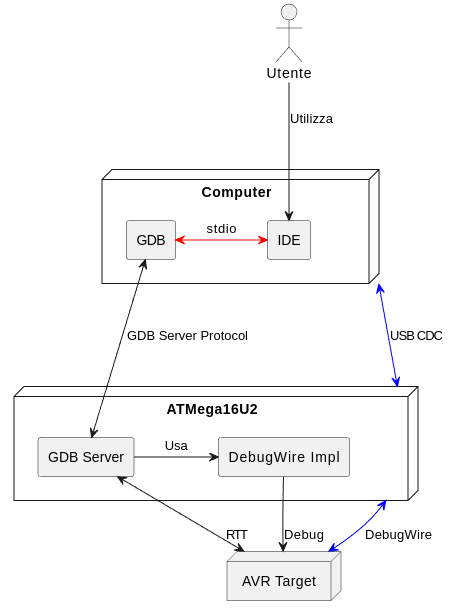
\includegraphics[width=.7\textwidth]{sys-arch.png}
    \caption[]{Diagramma dei componenti del sistema di assistenza alla programmazione e debugging}\label{fig:sys-arch}
\end{figure}

Come osservabile dalla figura~\ref{fig:sys-arch}, il sistema sviluppato si basa su tre livelli fisici collegati a cascata, in modo tale da adattare le azioni ad alto livello scelte dall'utente ai comandi di debug a basso livello che permettono di interagire con il controllore \textit{target}. 

Il primo livello, ovvero il livello di interfaccia con lo sviluppatore, consiste nel software utilizzato per lo sviluppo del firmware contenente tutti gli strumenti di supporto alla programmazione C. Questi software, anche noti IDE\footnote{Integrated Development Environment}, hanno il compito di accorpare svariate funzionalità mediante integrazione di software esterni allo scopo di favorire lo sviluppo fornendo un ambiente unico e integrato allo sviluppatore, dal quale effettuare tutte le operazioni quali sviluppo, compilazione, debugging e upload.

Enfasi particolare viene posta sull'integrazione da parte dell'IDE del software GDB.\@

Il \textit{debugging} è una delle pratiche ormai fondamentali della programmazione la quale permette una comprensione agevolata del flusso di esecuzione del codice e permette di ispezionarne i vari stati.

In particolare esso permette di analizzare uno stato intermedio tramite l'esecuzione in modo interattivo, consentendo allo sviluppatore di condurre ``un'indagine'' relativa a un funzionamento inatteso del firmware. Per citare un detto diffuso sulle piattaforme social in ambito di programmazione possiamo affermare che la procedura di \textit{debugging} sia paragonabile ad un'indagine condotta dallo sviluppatore dove egli stesso è il colpevole.

È necessario porre un'ulteriore enfasi sull'aggettivo ``interattivo'': la differenza tra \textit{debugging} e \textit{logging} sta proprio nel fatto che il secondo consiste nella stampa, su un terminale o file, di una serie di messaggi statici e predefiniti. Ciò non permette quindi di effettuare decisioni in funzione dei risultati parziali ottenuti nella procedura di \textit{debugging} a meno di riprogrammare il dispositivo --- inficiando così sulla longevità delle memorie --- e ricapitolare l'esecuzione del codice.

\section{Gnu Debugger}\label{sec:gdb}
\subsection{Debugging di dispositivi embedded}
%introduzione, architettura client server
\subsection{Integrazione con ambienti di sviluppo}

\section{GDB Server e Livello fisico}

Il secondo livello è costituito dal firmware presente sull'ATMega16U2 presente sulla scheda \textit{Arduino Uno R3} (componente \texttt{U3}).

Questo firmare, completamente ripensato rispetto all'originale, si occupa di convertire i comandi inviati dall'\textit{host} tramite una connessione USB simulando un dispositivo seriale e adattarli al debugging tramite DebugWire, implementando un server GDB direttamente all'interno dell'integrato.

Il secondo livello si occuperà di mantenere una connessione compresa di stato con il \textit{debugger}, ``tradurre'' i comandi GDB in modo che possano essere inoltrata al target tramite protocollo DebugWire e garantire funzionalità aggiuntive quali un livello di comunicazione \textit{target-to-host} su connessione di debug nominato Real Time Terminal (RTT).

Il firmware dell'ATMega16U2 è composto da quattro macro regioni descritte a seguire in questa relazione:
\begin{enumerate}
    \item Comunicazione USB con l'\textit{host}, implementata grazie all'utilizzo di una libreria esterna (LUFA\footnote{https://github.com/abcminiuser/lufa}).
    \item Server GDB
    \item Implementazione dell'interfaccia seriale open collector
    \item Implementazione del protocollo DebugWire
\end{enumerate}

